\documentclass{examen}

\begin{document}
\modulo{Lenguajes de marcas y sistemas de gesti�n de informaci�n}
\pregunta{
Una empresa desea modelar un flujo que indique las novedades en su canal de ventas, por lo que desea ver como quedar�a un archivo RSS que refleje dichas novedades.
\begin{itemize}
\item{La URL principal es http://acme.com y el canal de la empresa se llamar� ``Novedades de ACME'' siendo su descripci�n ``Las m�s recientes novedades al servicio de nuestros clientes''}
\item{Dentro de dicho canal se desea ver noticias de ejemplo}
\begin{enumerate}
	\item{La primera apunta a la URL http://acme.com/novedades1 su descripci�n es ``Disponible la nueva actualizaci�n de Android en los servidores de Google y r�plicas autorizadas`` y el t�tulo ``Nueva versi�n de Android''}
	\item{La segunda noticia tiene la URL http://acme.com/novedades2, su t�tulo es ``Fin de XP'' y la descripci�n es ``Finaliz� el soporte de Microsoft para Windows XP''}
\end{enumerate}

\end{itemize}

}{2.5}

\break 
\pregunta{Dado el archivo XML que se puede encontrar al final, 
crear una hoja de estilo XSLT que genere el HTML necesario para que se extraigan en forma de lista ordenada los datos (plataforma, cantidad de RAM y tama�o) de los tablets cuya RAM sea menor de 3.
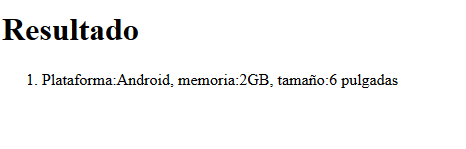
\includegraphics[scale=0.5]{examen-img/ejlistaordenada.png}
}{3}
\pregunta{Transformar el XML del pedido en el XML que se muestra al final. En concreto obs�rvese que se han dividido tablets y port�tiles en ``equipos con mucha RAM'' y ``equipos con poca RAM''. Se supone que un equipo con mucha RAM tiene 3GB o m�s. Los precios de los equipos no se muestran en el fichero final }{4.5}		

\break

\begin{lstlisting}{language=xml}
<!--FICHERO ORIGINAL-->
<pedido>
	<portatiles>
		<portatil>
			<peso>1430</peso>
			<ram unidad="MB">4096</ram>
			<disco tipo="ssd">500</disco>
			<precio>499</precio>
		</portatil>
		<portatil>
			<peso>1830</peso>
			<ram unidad="GB">6</ram>
			<disco tipo="ssd">1000</disco>
			<precio>1199</precio>
		</portatil>
		<portatil>
			<peso>1250</peso>
			<ram unidad="MB">2048</ram>
			<disco tipo="ssd">750</disco>
			<precio>699</precio>
		</portatil>
	</portatiles>
	<tablets>
		<tablet>
			<plataforma>Android</plataforma>
			<caracteristicas>
				<memoria medida="GB">2</memoria>
				<tamanio medida="pulgadas">6</tamanio>
				<bateria>LiPo</bateria>
			</caracteristicas>
		</tablet>
		<tablet>
			<plataforma>iOS</plataforma>
			<caracteristicas>
				<memoria medida="GB">4</memoria>
				<tamanio medida="pulgadas">9</tamanio>
				<bateria>LiIon</bateria>
			</caracteristicas>
		</tablet>
	</tablets>
</pedido>

\end{lstlisting}

\break

\begin{lstlisting}{language=xml}
<!--Fichero que debe salir como resultado del ejercicio 3-->
<pedido>
	<portatiles>
        <con_mucha_ram>
            <portatil>
                Portatil con 1430 g de peso, 4GB de RAM y 500GB de Disco SSD
            </portatil>
            <portatil>
                Portatil con 1830 g de peso, 6GB de RAM y 1000GB de Disco SSD
            </portatil>
        </con_mucha_ram>
        <con_poca_ram>
            <portatil>
                Portatil con 1250 g de peso, 2GB de RAM y 750GB de Disco SSD
            </portatil>
        </con_poca_ram>
	</portatiles>
	<tablets>
        <con_mucha_ram>
            <tablet>
                    Tablet iOS de 4GB, 9 pulgadas y bater�a LiIon
            </tablet>
        </con_mucha_ram>
        <con_poca_ram>
            <tablet>
                Tablet Android de 2GB, 6 pulgadas y bater�a LiPo
            </tablet>
        </con_poca_ram>
	</tablets>
</pedido>

\end{lstlisting}


\end{document}
